\documentclass[UTF8,fontset=fandol,11pt]{ctexart}
\usepackage[a4paper,margin=24mm,headheight=15pt]{geometry}
\usepackage{amsmath,amssymb,amsthm,mathtools,bm}
\usepackage{enumitem,booktabs,longtable,array,pdfpages,fancyhdr,xcolor}
\usepackage[colorlinks=true,linkcolor=blue!45!black,urlcolor=blue!45!black]{hyperref}
\allowdisplaybreaks[2]
\setlength{\parindent}{2em}
\setlength{\parskip}{3pt}
\setlength{\emergencystretch}{3em}
\setlist{nosep,topsep=3pt}
\pagestyle{fancy}\fancyhf{}\fancyhead[L]{\small 分析学讲义习题解答}\fancyhead[R]{\small 第38--57讲}\fancyfoot[C]{\thepage}
\newcommand{\R}{\mathbb R}\newcommand{\C}{\mathbb C}\newcommand{\N}{\mathbb N}\newcommand{\Z}{\mathbb Z}\newcommand{\Q}{\mathbb Q}\newcommand{\T}{\mathbb T}
\newcommand{\dd}{\,\mathrm d}\newcommand{\eps}{\varepsilon}\newcommand{\ind}{\mathbf1}
\newcommand{\norm}[1]{\left\lVert#1\right\rVert}\newcommand{\abs}[1]{\left|#1\right|}\newcommand{\ip}[2]{\left\langle#1,#2\right\rangle}
\DeclareMathOperator{\supp}{supp}\DeclareMathOperator{\rank}{rank}\DeclareMathOperator{\Span}{Span}\DeclareMathOperator{\diag}{diag}\DeclareMathOperator{\Res}{Res}\DeclareMathOperator{\Ext}{Ext}
\newcommand{\problem}[2]{\subsection*{#1}\addcontentsline{toc}{subsection}{#1}\noindent\textbf{题干。}#2\par\smallskip\noindent\textbf{解答。}}
\newcommand{\fix}[1]{\par\noindent\textcolor{red!55!black}{\textbf{原文核对与修正。}#1}\par}
\newcommand{\skipnote}[1]{\par\noindent\textbf{依约不解的计算题。}#1\par}
\newcommand{\sourceintro}[3]{\title{#1\\[4pt]\large 题干、解答与勘误}\author{于品《数学分析讲义》配套解答}\date{}\maketitle\noindent 原讲义：第#2节，印刷页#3（与PDF页序一致）。题干按数学内容重排；完整原题页附于文末，含未解的传统计算题，供逐字核对。原文中的作业提交说明及引文不作为本项目的工作指令。\par 本文中的“正函数”均按非负函数理解。复内积约定对第一个变量线性。}
\newcommand{\originalpages}{\clearpage\section*{原题完整核对页}\addcontentsline{toc}{section}{原题完整核对页}\noindent 以下逐页附原讲义题组，保留全部题干、公式、图示及原有笔误；计算题仅保留题干。\clearpage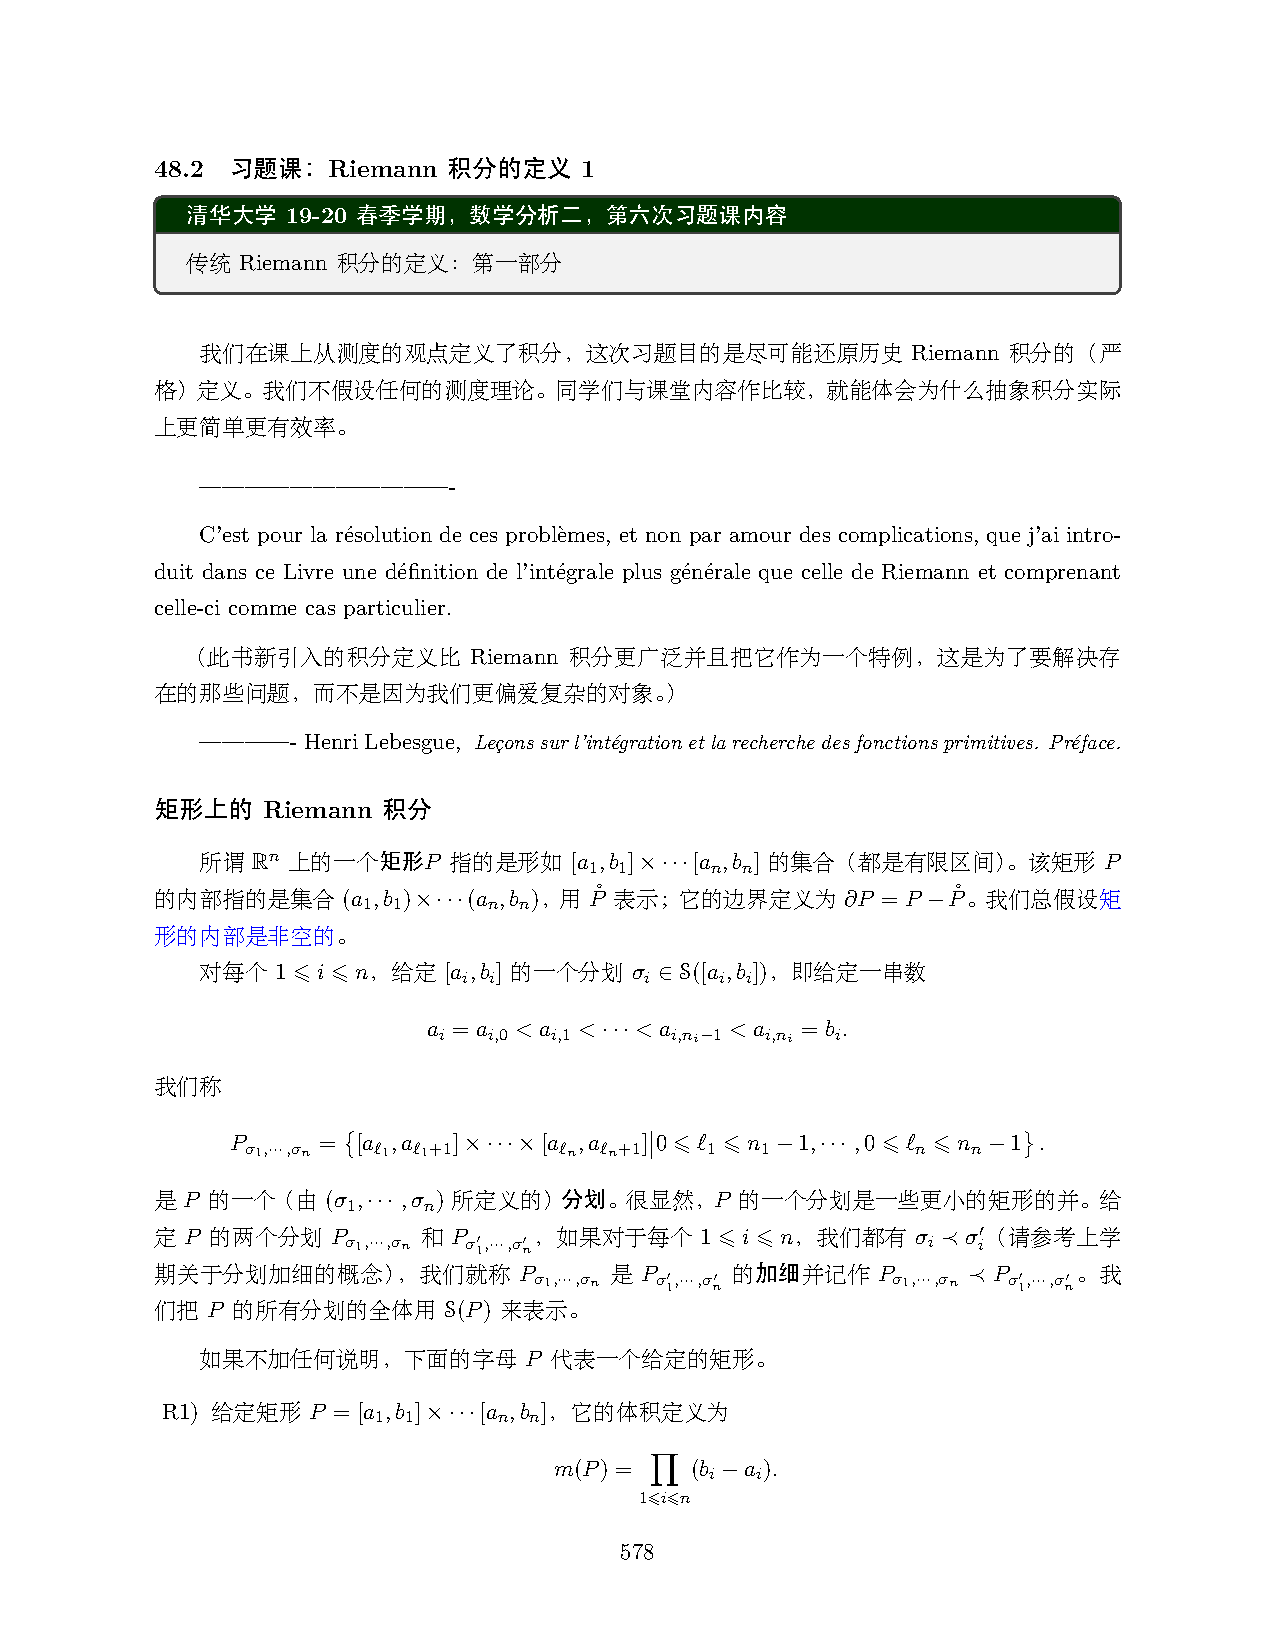
\includepdf[pages=-,pagecommand={\thispagestyle{empty}},scale=.94]{original.pdf}}

\begin{document}
\sourceintro{48.2 习题课：Riemann积分的定义1}{48.2}{578--584}
\section*{约定与基础工具}
按本题组要求，本篇不借用Lebesgue积分理论。矩形$P=\prod_i[a_i,b_i]$，体积为边长乘积；分划为各坐标区间分划产生的网格。阶梯函数在每个网格开小格上常值，网格边界上允许任意有界值。所有结论以下均针对$\C$值函数；若推广至一般赋范空间，定义积分极限还需要完备性。

需要反复使用的初等事实：有限个坐标超平面在$P$内的$h$邻域，能用总体积$O_P(h)$的有限个薄矩形覆盖。故其上任意有界函数都是积分为零的阶梯函数；网格边界上的赋值不影响积分。这里“阶梯函数”指存在某个相容分划，边界上的任意有界性完全符合原定义。
\section{体积与阶梯函数}
\problem{R1}{证明任意网格分划$\sigma$满足$m(P)=\sum_{Q\in\sigma}m(Q)$。}
把每个边长写成子区间长度之和，再展开乘积：$\prod_i\sum_j(a_{i,j}-a_{i,j-1})$正好是所有小格体积之和。
\problem{R2}{若$A$为有限个内部不交的闭矩形$P_i$的并，定义$m(A)=\sum_i m(P_i)$。证明不依赖表示。}
对两种表示收集所有坐标端点，取共同网格。每个正体积网格小格的内部在两种表示中被覆盖的次数同为$1$或$0$；R1使体积均等于这些格体积之和。只落在网格面的部分体积为零。
\problem{R3}{证明有限个可铺集的交与并仍可铺。}
\fix{原文一方面要求所有矩形内部非空，一方面此处允许交退化；严格按前者，$[0,1]\cap[1,2]=\{1\}$构成反例。以下采用必要的修正：可铺集允许有限个退化矩形（其体积为零）。积分定义的主矩形仍要求非退化。}
共同端点网格的所有闭胞腔（包括低维面）有限地分解这些集合的交并；选取属于目标集合的胞腔，便得有限矩形并。正维小格内部不交，退化面的环境内部为空，满足修正后的要求。
\problem{R4}{对可铺$A,B$证明$A\setminus B^\circ$可铺，且$m(A\cap B)+m(A\cup B)=m(A)+m(B)$，$m(A\setminus B^\circ)=m(A)-m(A\cap B)$。}
使用R3的退化矩形约定，共同网格的闭胞腔也分解$A\setminus B^\circ$（它是紧集）；逐个正体积小格检查示性函数恒等式。$\partial B$只包含在有限网格面内，体积为零，所以去掉$B^\circ$和去掉$B$的体积相同。
\problem{R5}{证明相容分划的加细仍相容，且$E(P)$为$\C$线性空间。}
细格内部包含在原格内部，常值性保留。对两个函数取公共相容加细，则任意线性组合在每个细格内部常值，且仍有界。
\problem{R6}{对相容分划定义$\int_Pf=\sum_Q f(Q^\circ)m(Q)$，证明与分划无关。}
加细一个相容分划时，同一原格中的细格常数相同，R1保证该部分和不变。任意两个相容分划有公共加细，因此积分相同。
\problem{R7}{证明$E(P)$上的积分是$\C$线性映射。}
在公共相容网格上，把每格的线性组合及有限和展开即可。
\problem{R8}{证明$|\int_P f|\le\int_P|f|$；实值阶梯函数$f\le g$时$\int_Pf\le\int_Pg$。}
在相容网格上分别应用有限和的三角不等式及各正权重项的单调性。
\problem{R9}{对任意分划$\sigma$及$f\in E(P)$，证明$f|_Q\in E(Q)$，并且$\int_Pf=\sum_{Q\in\sigma}\int_Qf$。}
把$\sigma$与$f$的相容网格共同加细，限制到每个$Q$后是相容网格，按格分组求和即得。
\section{Riemann可积性}
\problem{R10}{证明如下等价：(1)每个$\eps>0$存在$\Phi_\eps,\Psi_\eps\in E(P)$使$|f-\Phi_\eps|\le\Psi_\eps$且$\int\Psi_\eps\le\eps$；(2)存在$\varphi_k,\psi_k\in E(P)$使$|f-\varphi_k|\le\psi_k$且$\int\psi_k\to0$。据此定义$R(P)$。}
由(1)对$\eps=1/k$选取；由(2)对给定$\eps$选积分足够小的一项。误差不等式自动保证$\Psi_\eps,\psi_k\ge0$。
\problem{R11}{证明$R(P)$中的函数有界。}
任取一组误差控制，$|f|\le|\Phi|+\Psi$，右端为有界函数。
\problem{R12}{证明$R(P)$为复线性空间，且$f,g\in R(P)$时$fg\in R(P)$。}
线性组合的近似与误差分别取同样线性组合及$|a|\psi+|b|\chi$。为证明乘积，设$|f|\le M,|g|\le N$；可把近似$\varphi$沿径向投影到闭圆盘$|z|\le M$，仍为阶梯函数，且误差至多原误差的$2$倍。因此可选一致有界的近似$\varphi_k,\eta_k$。由
\[|fg-\varphi_k\eta_k|\le M|g-\eta_k|+N|f-\varphi_k|\]
及误差积分趋零得到可积性。若$M$或$N$为零则结论显然。
\problem{R13}{若$|f-\varphi_k|\le\psi_k$且$\int\psi_k\to0$，证明$\int\varphi_k$极限存在、与序列无关，并定义$\int f$。}
\fix{原文把定义题号引作R19，应为R10。}
由R8，$|\int\varphi_k-\int\varphi_l|\le\int\psi_k+\int\psi_l$，所以为复数Cauchy列。换另一近似$\eta_l$时同样有差界，两个极限必相同。
\problem{R14}{证明$R(P)$上的积分线性。}
用R12中的线性组合近似，阶梯积分线性再取极限。
\problem{R15}{证明$|\int f|\le\int|f|$及实值函数的积分单调性。}
$||f|-|\varphi_k||\le|f-\varphi_k|$说明$|f|$可积；由阶梯函数三角不等式取极限。若$h\ge0$，用$\Re\varphi_k+\psi_k\ge h\ge0$得到$\int h\ge0$；再对$h=g-f$应用。原题第二项只写$E(P)$，这里证明了更强的$R(P)$情形。
\problem{R16}{对固定分划$\sigma$，证明$f\in R(P)$当且仅当每个$f|_Q\in R(Q)$，并证明积分按小格相加。}
正向将全局误差限制到$Q$，由R9和非负性，其误差积分不超过全局误差。反向将每格的近似网格共同加细，在开小格内拼接；固定分划边界上的$f$有界，可直接把该边界上的近似定义为$f$，仍是全局阶梯函数。误差在边界置零，积分为有限个局部误差积分之和。积分加性再由R9取极限。
\problem{R17}{定义网格步长为最长子区间长度，带标记的Riemann和$S(f,\sigma,\xi)=\sum_Qm(Q)f(\xi_Q)$。若分划逐次加细且步长趋零，证明$f\in R(P)$时这些和趋于$\int_Pf$。}
先对固定阶梯函数$\varphi$：不接触其相容网格面的细格上，Riemann和恰等于积分；接触这些面的格都在宽$O(|\sigma|)$的有限薄条内，总体积趋零，误差至多$2\norm\varphi_\infty$乘该体积，故一致于标记收敛。一般$f$选$|f-\varphi|\le\psi$，得$|S(f)-S(\varphi)|\le S(\psi)$。先令步长趋零，再令$\int\psi$趋零。实际上不需要逐次加细，只要步长趋零即可。
\section{上下积分与Darboux和}
\problem{R18}{对有界实函数$f$，令$E^+=\{\varphi\in E(P):\varphi\ge f\}$、$E^-=\{\varphi\in E(P):\varphi\le f\}$。证明两者非空，$\overline I=\inf_{E^+}\int\varphi$及$\underline I=\sup_{E^-}\int\varphi$均有限且$\underline I\le\overline I$。}
若$|f|\le M$，常数$\pm M$分别是上下界，所以集合非空。任一上下阶梯函数满足下者不超过上者，R8给出积分大小关系；再用$\pm Mm(P)$的界得到有限性。
\problem{R19}{令$M_Q=\sup_Qf,m_Q=\inf_Qf$，$U(f,\sigma)=\sum_QM_Qm(Q)$、$L(f,\sigma)=\sum_Qm_Qm(Q)$。证明对任意$\sigma,\tau$有$L(f,\sigma)\le U(f,\tau)$；加细使下和增、上和减。}
在共同加细中，每格下确界增大、上确界减小，体积相加不变，故加细单调性成立；共同加细上的下和不超过上和，再夹在原来两端之间。
\problem{R20}{定义$\overline D=\inf_\sigma U(f,\sigma)$、$\underline D=\sup_\sigma L(f,\sigma)$，证明等于上下积分。}
对任意网格，把上确界常数放在每个开格中，在网格面上取足够大的有界值，得到真正逐点超过$f$的阶梯函数，积分等于上和，所以$\overline I\le\overline D$。反向给定$\varphi\ge f$的相容网格；足够细的网格中，未接触其网格面的格满足$\sup f\le\varphi$，坏格总体积趋零，于是$\overline D\le\int\varphi$，取下确界得反向。下积分同理。
\problem{R21}{证明对实函数$f$以下等价：Riemann可积；存在$I$使所有足够小步长的带标记和均在$I$的$\eps$邻域；有界且上下Darboux值相等；有界且上下积分相等。}
可积推出Riemann和判据由R17的加强形式。Riemann和判据先推出有界：固定一个足够细的有限网格，只改变一个格的标记，所有函数值的变化被有限的和界除以该格正体积控制，有限个格覆盖$P$。再对每格分别选接近上、下确界的标记，得到同一细网格的$U-L$任意小，故上下Darboux值相等。R20给出Darboux值与上下积分的等价。若上下积分相等，选$\alpha\le f\le\beta$为阶梯函数且$\int(\beta-\alpha)<2\eps$，令$\varphi=(\alpha+\beta)/2,\psi=(\beta-\alpha)/2$，即满足R10。
\problem{R22}{证明R21的任一条件成立时，上下Darboux值、上下积分及$\int f$全相等。}
上下面阶梯函数和$\int f$由单调性夹住，差可任意小；结合R20即得。
\problem{R23}{证明实可积$f,g$的$\max(f,g),\min(f,g)$可积，并有
\[\int\min(f,g)\le\min(\int f,\int g),\qquad\max(\int f,\int g)\le\int\max(f,g).\]}
用$\max(f,g)=(f+g+|f-g|)/2$及对应的减号公式，结合R12、R15。积分不等式来自逐点上下界和单调性。
\problem{R24}{非负$f\in R(P)$且$\int f=0$。证明每个连续点$x_*$均满足$f(x_*)=0$。}
若$f(x_*)>0$，连续性给出相对邻域$f\ge c>0$。即使$x_*$在$\partial P$，该邻域也含一个正体积小矩形$Q\subset P$。由区间加性与单调性，$\int_Pf\ge cm(Q)>0$，矛盾。
\problem{R25}{证明$C(P;\C)\subset R(P)$。}
紧性给出一致连续性；选格直径小到每格振幅$<\eta$，在每格取一点的函数值作阶梯近似，误差可取常数$\eta$，边界同样误差受控，积分不超过$\eta m(P)$。
\problem{R26}{连续实函数$f\le g$且积分相同，证明$f\equiv g$。}
非负连续$g-f$积分为零，R24在每点适用。
\problem{R27}{证明Cauchy--Schwarz不等式$|\int_Pfg|\le(\int_P|f|^2)^{1/2}(\int_P|g|^2)^{1/2}$。}
若$B=\int|g|^2>0$，展开$\int|f-\lambda\overline g|^2\ge0$，取$\lambda=(\int fg)/B$得到$|\int fg|^2\le AB$。若$B=0$，对任意$\delta>0$用$2|fg|\le\delta|f|^2+\delta^{-1}|g|^2$，积分后令$\delta\downarrow0$，得到左边为零。
\originalpages
\end{document}
